\documentclass[conference,letterpaper]{IEEEtran}
% Standard IEEE conference layout; no altered margins or reduced body font.
\usepackage[T1]{fontenc}
\usepackage[utf8]{inputenc}
\usepackage{amsmath}
\usepackage{newtxtext,newtxmath}
\usepackage{cite}
\usepackage{graphicx}
\usepackage{booktabs,tabularx,array}
\usepackage{microtype}
\usepackage{xcolor}
\usepackage{url}
\usepackage[hidelinks]{hyperref}
\usepackage{flushend}
\newcommand{\repositorylink}{\url{https://github.com/MohdMuzakkiruddinAhmed/traceable-entity-reconciliation}}

\newcommand{\ind}{\mathbf{1}}
\newcommand{\method}[1]{\textsc{#1}}
\newcolumntype{Y}{>{\raggedright\arraybackslash}X}
\hypersetup{pdftitle={Traceable Entity Reconciliation for Enterprise Knowledge Graphs: Context, Query Correctness, and Scale},pdfauthor={Muzakkiruddin Ahmed Mohammed; Shames AL Mandalawi; Abdelrahman Elfikky; John R Talburt},pdfsubject={IEEE KG-BigData 2026 workshop research manuscript}}
\graphicspath{{figures/}}
\begin{document}
\title{Traceable Entity Reconciliation for\\Enterprise Knowledge Graphs:\\Context, Query Correctness, and Scale}
\author{\IEEEauthorblockN{Muzakkiruddin Ahmed Mohammed, Shames AL Mandalawi,\\
Abdelrahman Elfikky, and John R Talburt}
\IEEEauthorblockA{Center for Advanced Research in Entity Resolution and Information Quality (ERIQ)\\
University of Arkansas at Little Rock\\
\href{mailto:mmohammed6@ualr.edu}{mmohammed6@ualr.edu}\qquad
\href{mailto:salmandalaw@ualr.edu}{salmandalaw@ualr.edu}\\
\href{mailto:aelfikky1@ualr.edu}{aelfikky1@ualr.edu}\qquad
\href{mailto:Jrtalburt@ualr.edu}{Jrtalburt@ualr.edu}}}
\maketitle

\begin{abstract}
Incorrect entity links can distort enterprise query answers even when ingestion and query execution are internally consistent. We present an auditable reconciliation architecture that preserves source observations, combines attributes with gated transaction context, and adds constrained canonical identities. Five linked evaluations separate source fidelity, matching quality, query accuracy, defect sensitivity and calibration, and computational scale across Wide World Importers (WWI), Olist, DataCo, BPI Challenge 2019, and all 27 WDC Products pairwise configurations. Three-seed mean conditional F1 changes by $+0.0200$, $+0.0923$, $-0.0212$, and $+0.4492$ on the four graph tasks, respectively; BPI compares detailed histories with coarse history descriptors. Independent SQL and graph extraction yield equal contextual scores. A paired postconstraint query evaluation finds identity-answer F1 of 0.802/0.832, 0.694/0.743, 0.790/0.747, and 0.063/0.528 for attribute/context maps, demonstrating task-dependent downstream effects. WDC is an attribute-only reference: a frozen embedding cosine increases fully unseen mean F1 from 0.5369 to 0.5584. Forty-five scaling trials complete, with substantial retrieval losses under replication. The contribution is an inspectable architecture and controlled evaluation of evidence, identity decisions, and query consequences. The results establish conditional benefits and explicit failure modes within the evaluated tasks.
\end{abstract}

\begin{IEEEkeywords}
entity resolution, enterprise knowledge graphs, transaction context, provenance, query correctness, reproducible evaluation
\end{IEEEkeywords}

\section{Introduction}
Enterprise integration requires agreement about identity as well as agreement about schema. Purchasing, inventory, finance, and customer systems can describe the same supplier, product, or customer using different identifiers and lexical forms. Leaving those observations disconnected omits valid cross-source paths. Merging different entities creates a more subtle failure: the system can return a coherent, reproducible answer about the wrong entity. Entity reconciliation is therefore both a matching problem and a data-management decision whose consequences should remain inspectable.

Attributes such as names, categories, and product descriptions provide an initial matching signal. Local histories can add observations about categories, activities, timing, and compatible quantities. However, two different products can share suppliers, and two different customers can exhibit similar purchasing behavior. More contextual evidence is not necessarily more informative evidence. Moreover, representing a history as a knowledge graph does not establish that its storage format improves prediction. The contribution of information must be distinguished from the contribution of its representation.

This paper examines that distinction through an auditable enterprise reconciliation prototype. Typed source observations and lineage remain intact; matching uses a restricted source-view projection; and canonical identities are added only after scoring. A binary support gate determines whether a candidate receives a contextual or attribute score. Independent relational controls test source fidelity, reproduce the permitted contextual features, and execute queries under the same identity maps as the graph implementation. This arrangement permits a reconciliation error to be distinguished from an extraction or query-implementation error.

\subsection{Research Position and Contributions}
Collective entity resolution exploits relationships among references~\cite{bhattacharya2007}; GraphER combines graph differential dependencies with neural processing~\cite{grapher2025}; and Ditto learns pair classification with pretrained language models~\cite{ditto2020}. Sentence-BERT and MiniLM motivate our frozen single-cosine reference~\cite{sbert2019,minilm2020,minilmcard}. These approaches motivate contextual and learned evidence. Table~\ref{tab:position} distinguishes their methodological emphasis from the controls implemented here; it is not a performance comparison.

\begin{table}[t]
\caption{Research position: reference emphasis and the corresponding control in this study. Listed controls describe this artifact, not an exhaustive audit of prior systems.}
\label{tab:position}
\centering\small
\setlength{\tabcolsep}{3pt}
\begin{tabularx}{\columnwidth}{@{}p{.22\columnwidth}YY@{}}
\toprule
Reference & Emphasis & Control here\\
\midrule
Collective ER~\cite{bhattacharya2007} & Relational evidence and joint resolution & Fixed source views; no canonical feedback\\
GraphER~\cite{grapher2025} & Dependencies and neural graph matching & Engineered context; SQL feature/score parity\\
Ditto~\cite{ditto2020} & Learned language-model pair matching & Equal learner catalogs; frozen cosine reference\\
LIS / PROV-O~\cite{lis2023,provo2013} & Typed integration and provenance & Source/decision lineage; oracle query controls\\
\bottomrule
\end{tabularx}
\end{table}

The methodological problem addressed here is \emph{attribution}: improved pair F1 alone does not identify whether the benefit comes from additional evidence or graph storage, whether accepted identities improve business queries, or whether retrieval losses negate the gain. We address these questions in one controlled pipeline. Blocking research motivates candidate-aware denominators~\cite{blocking2020}; WDC supplies complementary product-offer tasks with varying difficulty, size, and unseen entities~\cite{wdc2024}. LIS and PROV-O motivate typed integration and explicit origins~\cite{lis2023,provo2013}. This property-graph artifact follows a design-science evaluation perspective~\cite{hevner2004}.

We make three contributions. \emph{First}, we implement source-preserving ingestion and lineage with a separate, constrained canonical view. \emph{Second}, we evaluate gated context on common candidates with equal learner catalogs and independent relational extraction controls. \emph{Third}, we compare attribute and contextual identity maps through oracle-based query answers and link these outcomes to defects, calibration, and retrieval-aware scale. This is a systems and evaluation contribution; the learned references are not reproductions of GraphER or Ditto.

RQ1 concerns source relationships and lineage; RQ2 contextual matching benefit; RQ3 identity-dependent query accuracy and SQL/graph agreement; RQ4 defects and decision reliability; and RQ5 computational and retrieval trade-offs. E1--E5 address these questions. WWI and WDC were primary datasets; Olist, DataCo, and BPI expanded an exploratory study, including a test-informed Olist adapter amendment.

\section{Enterprise Reconciliation Scenario}
\label{sec:scenario}
Consider the evaluated procurement--inventory scenario in WWI. A purchasing view contains suppliers, purchase orders, and order lines. A warehouse/finance view contains stock observations, movements, and supplier transactions. Independently named master records prevent direct cross-view identity joins. A purchasing stock item that is not linked to its warehouse observation loses downstream paths; an incorrect link can attribute movements or supplier-related evidence to another product. Native foreign keys are retained only where the source supports them: no transaction-to-order relationship is invented to make a query answerable.

The knowledge graph separates three layers. The \emph{source layer} retains typed observations, their valid relationships, and their table and row origins. The \emph{matching projection} exposes only permitted local attributes and histories. The \emph{decision view} connects accepted source observations to generated canonical entities while retaining rejected, abstained, and conflicting candidates in the audit. Thus an identity decision adds an interpretation of the source data; it does not overwrite the source record. Figure~\ref{fig:architecture} shows this separation and the independent controls.

This scenario motivates two different correctness questions. Given a fixed identity map, SQL and graph execution should produce the same source-normalized answer. Given an evaluator oracle, the predicted identity map should produce the correct answer. The first can hold while the second fails. For example, both engines can agree on a transaction aggregation that has been attached to the wrong product. An oracle comparison is therefore necessary in addition to representation parity.

Olist, DataCo, and BPI instantiate related but distinct integration scenarios: repeated customer accounts, controlled customer aliases with partitioned orders, and vendor observations with partitioned purchase cases. These datasets broaden the kinds of evidence examined without turning the study into a common business-outcome benchmark. WDC contributes product-offer matching without transaction relationships. The application scope is traceable data integration and query attribution, not measured cost savings, financial loss, customer profiling effectiveness, or production process improvement.

\begin{figure*}[t]
\centering
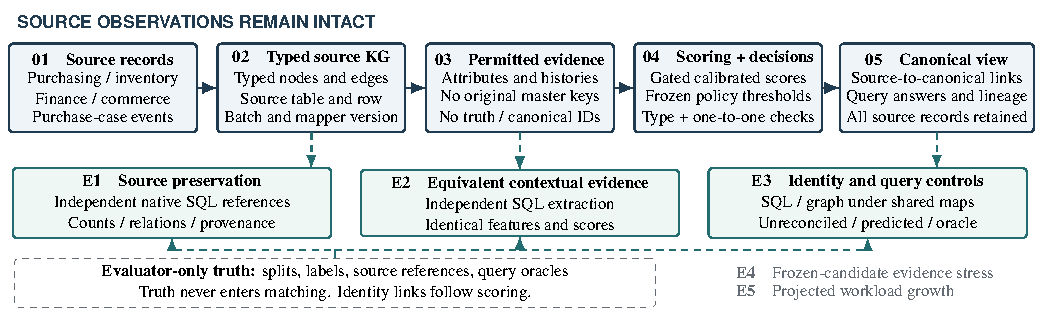
\includegraphics[width=\textwidth]{architecture.pdf}
\caption{Source-preserving enterprise reconciliation and independent controls. Solid arrows carry observed data or decisions. Dashed arrows lead to evaluation checks, not matching features. Evaluator truth is confined to splits, labels, reference checks, and query oracles. E4 perturbs permitted evidence with frozen candidates and models; E5 measures projected workloads. The diagram covers the four graph tasks; WDC is an attribute-only reference without an ERP transaction or query workload.}
\label{fig:architecture}
\end{figure*}

\section{Proposed Framework}
\label{sec:framework}
\subsection{Identity, Typed Ingestion, and Permitted Evidence}
Let $R_A$ and $R_B$ be records from two independently named source views, with type $t(r)$ and local identifier $u(r)$. Evaluator-only original identity $z(r)$ defines the target for a same-type cross-source pair:
\begin{equation}
y_{ab}=\ind[z(a)=z(b)].
\label{eq:truth}
\end{equation}
Original master keys, $z$, and postdecision canonical identifiers are excluded from matching features. Local identifiers address nodes and deterministically order ties; they do not enter matching text. Group identity remains available to the evaluator for splits, labels, and reference answers.

A typed property graph $G=(V,E)$ stores the declared record kinds, relation labels, and provenance. The expanded native graphs are SQLite-backed; the original WWI graph and matching projections use NetworkX. Generic projections expose \texttt{Master--Transaction--Category} paths. WWI additionally preserves typed master relations. Native imports can be much larger than the populations used for learning, and successful ingestion does not imply that every imported record trained a matcher.

Ingestion checks counts, valid endpoints, lineage presence, and repeated-edge-import idempotence. Independent native SQL joins define the expected relationship sets. Olist explicitly represents postal-prefix grouping rather than treating repeated geolocation observations as one unique coordinate. DataCo retains all row observations and normalization disagreements even though its master normalization uses first source occurrence. BPI preserves original trace ordinal for event ordering, including timestamp ties and inversions.

Lineage completeness is
\begin{equation}
q(r)=\frac{1}{3}\sum_{f\in\{\mathrm{table},\mathrm{batch},\mathrm{mapper}\}}
\ind[f(r)\text{ is present}].
\label{eq:lineage}
\end{equation}
The source row identifier is retained separately. Summary weights use the smaller completeness of a master and its local transaction; WWI anchor contributions also use visible attribute completeness. This is a metadata-availability measure, not an estimated probability of source correctness. A misleading edge can retain complete provenance.

\subsection{Attributes and the Frozen Embedding Reference}
The common attribute comparator has 20 features covering normalized character and token-sort similarity, token Jaccard, training-only character TF-IDF cosine, category/brand agreement, description similarity, price/currency compatibility, missingness, numeric/alphanumeric token overlap, size compatibility or conflict, name-length ratio, and digit missingness. WWI adds packaging equality, ratio, and missingness, giving 23 features. TF-IDF is fitted only on training records and sparse cosine computation is chunked. The common learners use scikit-learn~\cite{sklearn2011}.

Attribute price features do not convert currencies. Two empty currency strings count as equal in this implementation, so compatibility is not restricted to verified currencies. Contextual numerical features instead track declared unit classes and missing or incompatible units. In WWI, \texttt{QuantityPerOuter} converts purchased stock-item outer quantities to stock units and is also visible to learned attribute comparators. Signed stock movements, supplier-level outer quantities, and missing finance quantities remain distinct.

The neural reference uses the pinned \texttt{all-MiniLM-L6-v2} encoder~\cite{minilmcard}: CPU quantized ONNX inference, batch size 64, 256-token limit, attention-mask mean pooling, and L2 normalization. Allowed name/brand/description text is truncated to 2,000 characters before tokenization; IDs, truth, canonical keys, and prices are excluded. Each 384-dimensional embedding contributes one pair cosine. Embedding-only learning uses that scalar; augmented attributes concatenate it with lexical features. The encoder is not fine-tuned.

\subsection{Context Summaries and Support Gating}
Generic context has 16 dimensions: category/activity cosine, degree similarity, distinct shared tags, weighted support, date mean/span similarity, quantity and amount mean/deviation similarity, date availability, quantity/amount unit compatibility, category contradiction, and context availability. Moments are lineage-weighted. The generic support gate requires at least two distinct projected category tags and weighted support of at least one. Missing-value prefix tags can contribute, so passing this test does not guarantee two known informative categories or independently resolved entities.

WWI combines five native master-context dimensions with 15 transaction-summary dimensions. Its independent anchors are unique exact normalized names with compatible types and categories, excluding the candidate endpoints. Stock-to-supplier and co-supplied-stock paths provide typed context. At least two distinct inferred master anchors and weighted support of one are required. Packaging is excluded from anchor inference, although attribute comparison and contextual quantity conversion can use it.

For calibrated attribute probability $p_A$, contextual probability $p_C$, attribute vector $x$, contextual vector $c$, and binary support $h$, scoring is
\begin{equation}
p_G(a,b)=h_{ab}p_C(x_{ab},c_{ab})+(1-h_{ab})p_A(x_{ab}).
\label{eq:gate}
\end{equation}
When $h=0$, the score equals the attribute score exactly. This is not an equal-decision guarantee because methods retain separately selected acceptance thresholds. Nor does $h=1$ guarantee that context is correct or independent. Figure~\ref{fig:decision} distinguishes scoring from subsequent acceptance.

A separate flat SQL extractor independently joins the same permitted projection. If SQL and graph extraction produce equal $(x,c,h)$, the shared estimator, calibrator, and policy must yield equal scores. This is a representation-invariance control: measured predictive gains concern the supplied evidence, not graph storage itself. It is distinct from E1's native-source SQL fidelity checks.

\begin{figure}[t]
\centering
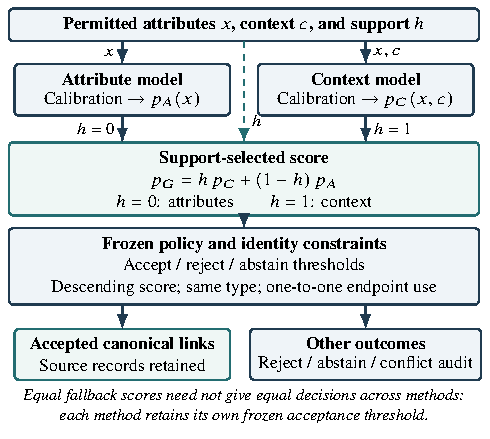
\includegraphics[width=\columnwidth]{decision_flow.pdf}
\caption{Gated scoring and constrained identity decisions. Unsupported pairs receive the attribute score; a method-specific frozen policy still governs decisions. Only accepted, type-consistent, nonconflicting links enter the canonical view. All outcomes retain source references and decision evidence.}
\label{fig:decision}
\end{figure}

\subsection{Non-Destructive Canonicalization}
Candidates are processed in descending score order using frozen acceptance thresholds, same-type constraints, and one-to-one endpoint use. Accepted observations point to added canonical entities through \texttt{REFERS\_TO} links; accepted cross-source links are recorded as \texttt{ACCEPTED\_SAME\_AS}. Rejected, abstained, and conflicting candidates remain auditable. Decisions retain source identifiers, scores, thresholds, model checksums, evidence references, and triggers. No canonical link feeds back into feature extraction.

The canonical layer is deliberately limited to two source views with at most one accepted partner per endpoint. It is not a transitive clustering algorithm for arbitrary within-source duplicates or multi-source identity groups. Traceability makes decisions inspectable and replayable; it does not establish that an accepted merge is harmless or that a human can interpret its evidence effectively.

\section{Experimental Methodology}
\label{sec:methods}
\subsection{Datasets and Application-Specific Identity Tasks}
Table~\ref{tab:datasets} separates native graph sizes from matching groups. Each group supplies two source-view observations; graph-node counts are not training-record counts. Alias/training seeds are 17, 29, and 43. Generic splits use stable hashing with seed 20261012; the validation-role seed adds 101. WWI retains its original split.

\begin{table*}[t]
\caption{Native ingestion and matching populations. WDC is offer-only and is described separately. Groups are original matching entities, not graph nodes.}
\label{tab:datasets}
\centering
\begin{tabular}{lrrrl}
\toprule
Dataset & Native nodes & Native edges & Matching groups & Train / validation / test groups\\
\midrule
WWI & 249,786 & 274,856 & 240 & 143 / 48 / 49\\
Olist & 1,569,937 & 1,775,243 & 2,913 & 1,747 / 583 / 583\\
DataCo & 267,103 & 607,478 & 1,500 & 900 / 300 / 300\\
BPI2019 & 1,926,659 & 7,138,894 & 1,378 & 826 / 276 / 276\\
\bottomrule
\end{tabular}
\end{table*}

\emph{WWI} is Microsoft's fictional business sample~\cite{wwi}. Six in-scope native tables supply the fidelity graph. Matching retains 13 suppliers and 227 stock items with controlled aliases in purchasing and warehouse/finance views. The matching views retain relevant purchase and supplier-transaction rows and the first 5,000 primary-key-sorted movements; E1 checks the complete in-scope movement table. The fixed test set contains 49 entities, including only three suppliers. Seeds vary aliases rather than independent populations.

\emph{Olist} uses all nine official version-2 CSVs~\cite{olist}. All 2,913 eligible repeated-customer groups have two distinct observed accounts with item histories; \texttt{customer\_unique\_id} is evaluator-only. Account selection is deterministic when more than two observations exist. Visible customer attributes are city, state, and postal prefix, not names. Up to 40 order items per view supply price and item-row count, with declared order/product/seller joins. Seller-state paths were added after a test-context diagnostic found no supported candidates using product categories alone, before expanded model fitting. This adapter development is partly test-informed and explicitly exploratory.

\emph{DataCo} uses the version-5 structured CSV, with 180,519 rows and 53 columns, not its clickstream data~\cite{dataco}. Publisher acquisition returned HTTP 403; a documented mirror supplies the hashed file, without established publisher-byte equivalence. Stable pre-alias hashing selects 1,500 of 10,075 eligible customers. Controlled name defects and disjoint order histories create the two views; native names, segment, and location are permitted, while email/password fields are excluded. This is not independently annotated naturally dirty identity data.

\emph{BPI Challenge 2019} provides 251,734 cases and 1,595,923 events; the publisher MD5 is checked~\cite{bpi}. All 1,378 eligible vendors supply partitioned purchase-case histories. Vendor names, vendor IDs, company identifiers, and original keys are excluded from matching text. Interface fields called name/category/brand instead contain modal spend-area, document-type, and spend-classification descriptors derived independently per view. Thus detailed context is compared with coarse history, not a supplier-name matcher. Quantity is unavailable; amount is the first-event anonymized cumulative case value, not summed cumulative events or actual payments. Generic histories are capped at 40 transactions/cases per view.

\emph{WDC Products} retains all 27 official hardness/development-size/unseen configurations~\cite{wdc2024,wdcdownloads}. The used pairwise files contain 155,957 pair observations, 10,422 offers, and 1,600 labelled groups, distinct from whole-benchmark counts. Each official test has 4,500 pairs and 500 positives. Nine hardness/size settings and three seeds produce 27 fitted bundles reused over three unseen variants, giving 81 evaluations, not 81 independent fits. The used-file audit flags training-test and/or validation-test offer intersections in 18 configurations. Fully unseen cells have no such intersections; a separate offer-disjoint diagnostic subset retains its own denominators. No transaction graph or ERP query workload is constructed for WDC.

\subsection{Candidates, Model Development, and Comparators}
Original entity groups are split before alias construction. Generic training/validation/test proportions are 60/20/20. Validation groups are further partitioned into selection, calibration, and policy roles; a pair enters a role only when both endpoints belong to that role. Cross-role pairs are omitted. Role weights restore full-validation candidate prevalence, using $\pi/\pi_r$ for positives and $(1-\pi)/(1-\pi_r)$ for negatives. This is not correction to a known test or deployment prior.

Every learned family compares five estimators: standardized class-balanced logistic regression with $C=0.1,1,10$ and class-balanced 160-tree random forests with depth 8 or 16 and minimum leaf size two. Logistic iteration limit is 1,500; forests use two jobs. Selection maximizes its own weighted F1, with catalog-order tie breaking. A separate role fits sigmoid calibration by logistic regression on logits of probabilities clipped to $[10^{-6},1-10^{-6}]$, with $C=10^6$ and iteration limit 1,000. The policy role chooses the acceptance threshold by weighted F1, preferring the higher threshold on ties. Rejection is bounded by 0.10 and acceptance. Models, calibrators, thresholds, and hashes are saved before test-label scoring.

E2 preserves WWI's original token-prefix/category block without a per-left $K$ cap, under a two-million-pair guard. Generic graph tasks use the common bounded $K=32$ pool. A candidate is ambiguous when normalized character similarity is below 0.95 or its left record has more than one candidate with token-sort similarity at least 0.65. All methods use this same diagnostic stratum. WDC E2 uses the official test pairs rather than a newly generated candidate set.

Exact matching requires nonmissing normalized-name equality and category agreement; fuzzy matching uses token-sort similarity. Learned references are attributes, embedding-only, and augmented attributes. Flat SQL context and gated graph context share the contextual estimator and policy. \method{NoContext} shares the attribute score and threshold. \method{NoGate} applies the weighted contextual learner without fallback using its own policy, rather than retraining a gate-free learner. \method{NoSupport} retrains without explicit support inputs but keeps the gate. Generic \method{OneHop} removes category traversal; WWI also transforms native master context. \method{NoTransactions} removes all 15 WWI transaction dimensions but only date/numeric/unit dimensions in generic adapters, retaining category/activity/degree evidence. \method{UnitWeights} changes inputs to the frozen weighted model and policy; it is a stress contrast, not a retrained provenance ablation.

\subsection{Five Linked Evaluations and Their Denominators}
\emph{E1} checks full in-scope source counts, relationship-set equality against native SQL, lineage, dangling endpoints, and idempotence. WDC checks offer identity, schema/counts, evaluator-label exclusion, and split-member hashes instead of ERP relations.

\emph{E2} evaluates 12 graph seed runs with 13 methods and 81 WDC cells with five methods. Let $C$ be candidates and $T$ the full set of true cross-source pairs. Blocking recall is $|C\cap T|/|T|$. Candidate-conditioned recall considers retained positives, whereas full-pipeline recall includes omitted positives. Before one-to-one constraints,
\begin{equation}
F_{1,\mathrm{end}}=\frac{2TP}{TP+FP+|T|}.
\label{eq:endf1}
\end{equation}
No scorer can recover a positive absent from $C$. Accepted-link errors are audited after constraints and use a different denominator. Per-seed paired bootstrap summaries resample original groups in ambiguous candidates 1,000 times. A same-group pair receives multiplicity $m_g$ and a distinct-group pair receives $m_gm_h$, with identical weights for both classifiers. Percentile endpoints 2.5/97.5 describe the paired F1 difference. Shared populations, three seeds, and correlated pairs preclude a pooled confirmatory interpretation.

\emph{E3} executes eight adapted query templates under unreconciled, predicted, and oracle identities. Source UIDs normalize tuples, and SQL/graph answers must agree under each map. Q2/Q4 are source-local controls; the other six depend on reconciliation. Amounts are cent-rounded source units; DataCo/Olist currency is unspecified and BPI values are anonymized case amounts. WWI additionally retains eight native purchasing, stock, finance, and provenance templates. The four adaptations are not 32 independent business workloads.

\emph{E4} freezes clean candidates, models, and policies across 12 graph conditions: clean, absent anchors/support, additional attribute noise 30/50\%, optional missingness 10/30/50\%, edge removal 15/30\%, typed misleading rewiring 15/30\%, and lineage missingness 30\%. Rewiring stays within entity kind, silo, and split; perturbation logs remain evaluator-only. WDC has six attribute-only conditions. Raw/calibrated Brier score, log loss, and ten equal-width-bin expected calibration error (ECE) assess reliability separately from discrimination~\cite{calibration2005}. Coverage and selective risk concern accepted/rejected pairs before one-to-one constraints. Retrieval is not rerun under corruption.

\emph{E5} uses targets of 1,000, 10,000, and 100,000 projected graph nodes or WDC offers, with three trials each: 45 main trials. Validation chooses $K\in\{8,16,32\}$ for a 0.95 recall target, with at most 12 keys, posting cap $8K$, and two-million emitted-pair guard. Hash-ordered postings and visible name similarity determine retrieval. WWI chooses $K=8$; generic tasks choose 32 without reaching the validation target. Later workload growth uses replicas, with all cross-replica positives in the matching denominator and no copy-suffix feature. Timed queries instead use a common per-copy oracle identity map. One warmup and five measured executions produce per-trial p50/p95; graph and SQL preparation are timed separately. RSS is sampled every 50\,ms. Hardware is Windows 11, 24 logical CPUs, approximately 63.46\,GiB RAM, and Python 3.12.10; these are local measurements.

\section{Results and Discussion}
\label{sec:results}
\subsection{E1: Fidelity of the Declared Source Mappings}
All four native graph imports match the expected in-scope relationship sets, retain complete measured lineage, have no dangling edges, and pass repeated-edge-import idempotence. WWI checks eight independent foreign-key controls, Olist ten native/derived relations, DataCo six, and BPI eight. These results support RQ1 within the declared mappings, exceeding the original 99\% relationship target. They do not prove publisher-data correctness or coverage of every possible business interpretation. WDC verifies its offer/pair structure rather than native ERP graph relations.

\subsection{E2: Conditional Contextual Benefit and Remaining Errors}
Table~\ref{tab:matching} reports three-seed mean F1 on common ambiguous candidates. Context changes WWI from 0.7688 to 0.7888, Olist from 0.6919 to 0.7842, DataCo from 0.6962 to 0.6750, and BPI from 0.1242 to 0.5734. The differences are $+0.0200$, $+0.0923$, $-0.0212$, and $+0.4492$. DataCo contradicts universal contextual improvement. Olist exact matching reaches 0.7502, above the learned attribute reference, so learned attributes are not the strongest noncontextual control on every task.

\begin{table}[t]
\caption{Three-seed mean F1 on common ambiguous candidates. These are conditional pair results, not full-pipeline or postconstraint metrics. Ablation semantics differ by adapter as specified in Section~\ref{sec:methods}.}
\label{tab:matching}
\centering
\small
\setlength{\tabcolsep}{3.4pt}
\begin{tabular}{lrrrr}
\toprule
Method & WWI & Olist & DataCo & BPI\\
\midrule
Exact & .3402 & .7502 & .1994 & .0538\\
Fuzzy & .7145 & .1039 & .2001 & .0639\\
\textbf{Attributes} & .7688 & .6919 & .6962 & .1242\\
Embedding & .4157 & .2327 & .2594 & .0840\\
Attributes + embedding & .7626 & .7414 & .6962 & .1492\\
Flat SQL context & .7888 & .7842 & .6750 & .5734\\
\textbf{Gated graph context} & .7888 & .7842 & .6750 & .5734\\
\midrule
No context & .7688 & .6919 & .6962 & .1242\\
No gate & .7763 & .7806 & .6710 & .5734\\
No support features & .7879 & .7913 & .6780 & .5465\\
No transaction summaries & .7887 & .7474 & .6790 & .4264\\
One hop & .7688 & .6919 & .6946 & .4827\\
Unit-weight inputs & .7440 & .7842 & .6750 & .5734\\
\bottomrule
\end{tabular}
\end{table}

Figure~\ref{fig:effects} exposes seed heterogeneity. WWI has one zero-effect seed and two small positive effects, with wide uncertainty relative to its average. Olist varies from $+0.0252$ to $+0.2043$; its seed-17 interval crosses zero. All DataCo point estimates are negative and their intervals cross zero. BPI's three positive intervals exclude zero under the specified resampling, but this contrast compares detailed histories with coarse modal descriptors. It cannot establish an analogous gain over literal vendor-name matching. These exploratory intervals are not pooled or multiplicity-adjusted hypothesis tests.

\begin{figure}[t]
\centering
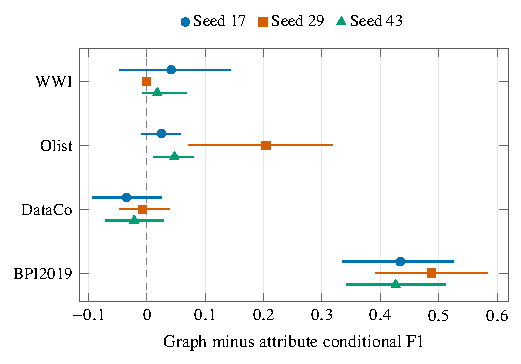
\includegraphics[width=\columnwidth]{context_effects.pdf}
\caption{Graph-minus-attribute conditional F1 with per-seed paired group-resampling percentile endpoints. Markers identify the three seeds; they reuse original source populations. The large BPI effects are conditional on its coarse history-derived baseline.}
\label{fig:effects}
\end{figure}

Flat SQL and graph context features and scores agree within $10^{-12}$, giving identical F1. This supports evidence equivalence, not graph-specific predictive superiority. Clean generic lineage weights are all one, so identical \method{UnitWeights} results there cannot establish that provenance weighting improves accuracy. WWI differs because its anchor-attribute completeness varies.

Table~\ref{tab:pipeline} reports the separate retrieval and final-decision consequences. Generic blocking omits positives even before classification: mean recall is 0.821 for Olist, 0.874 for DataCo, and 0.755 for BPI. End-to-end context F1 is therefore 0.725, 0.649, and 0.490, respectively, compared with 0.826 for WWI. The contextual benefit remains positive for WWI/Olist/BPI and negative for DataCo in this setup. After one-to-one constraints, false merges persist in every dataset. Accepted counts are sums over seed trials, not independent production events.

\begin{table*}[t]
\caption{Retrieval and full-positive-universe pair F1 before constraints; final gated-context links and precision/recall after constraints. Accepted/false counts and postconstraint precision/recall use totals over three shared-population seed trials. Preconstraint F1 and blocking recall are seed means.}
\label{tab:pipeline}
\centering\small
\begin{tabular}{lrrrrr}
\toprule
Dataset & Block recall & Attr. pair F1 & Ctx. pair F1 & Context accepted / false & Context link P / R\\
\midrule
WWI & 1.000 & .797 & .826 & 107 / 1 & .991 / .721\\
Olist & .821 & .654 & .725 & 1,092 / 37 & .966 / .603\\
DataCo & .874 & .674 & .649 & 636 / 62 & .903 / .638\\
BPI2019 & .755 & .110 & .490 & 372 / 54 & .855 / .384\\
\bottomrule
\end{tabular}
\end{table*}

\subsection{WDC: Attribute Generalization and Split Auditing}
On nine fully unseen configurations and three seeds, mean F1 is 0.0000 for exact matching, 0.3477 for fuzzy matching, 0.5369 for attributes, 0.3919 for embedding-only, and 0.5584 for augmented attributes. The scalar cosine adds 0.0215 to the descriptive attribute mean but is weaker alone. This is not an ERP context result or evidence of superiority to a fine-tuned pair model.

The benchmark paper describes offer-disjoint splits~\cite{wdc2024}. Our independent audit of the retained official pairwise archives finds offer-ID intersections in the files used for this study. IDs are compared across either pair endpoint, and every intersecting offer has identical cluster and attribute fields. For 20\% corner cases, small development size, and 50\% unseen entities, training/test and validation/test intersections contain 97 and 105 offers; the offer-disjoint diagnostic retains 2,918 of 4,500 test pairs. At 0\% unseen, the corresponding counts are zero and four; at 100\% unseen, both are zero. The revision supplement provides all 27 cells, exact member names, archive and decompressed hashes, hashed overlap examples, and the executable parser. The audit attributes this discrepancy to these retained files; its cause is unresolved. Some 0\%-unseen cells have zero training-test overlap but nonzero validation-test overlap, so checking training alone is insufficient. The 18 flagged configurations remain descriptive results; fully unseen and separately denominator-preserving offer-disjoint subsets supply cleaner diagnostics. Sizes reuse test pools, and means across configurations are correlated. No unseen variant is selected by test performance, and no pooled confidence interval is attached to the WDC headline.

\subsection{E3: Matching-to-Query Effects and Execution Parity}
All 288 original adapted query rows pass SQL/graph equality; the separate native WWI controls contribute 72 rows. Every oracle workload is nonempty. This revision adds a paired comparison of \emph{attribute-only} and \emph{gated-context} identity maps: four datasets $\times$ three seeds $\times$ two methods $\times$ eight queries give 192 freshly executed method/query cells. Frozen scores and each method's original validation-selected threshold are used with identical descending-score, same-type, one-to-one rules. The source projection, candidate pool, query templates, and oracle remain fixed. Contextual links and all 96 contextual query metrics exactly reproduce the saved study outputs. No learner or policy is refitted.

Table~\ref{tab:queries} reports arithmetic means of paired seed results. Q6 identity-answer F1 changes by $+0.030$ on WWI, $+0.048$ on Olist, $-0.043$ on DataCo, and $+0.465$ on BPI. All six identity-sensitive template means improve on Olist and BPI and decline on DataCo. WWI improves on five, but Q5 transaction-link F1 falls from 1.000 to 0.998: the additional false link slightly worsens transaction attribution. Thus a matching gain need not improve every downstream query. BPI's gain remains conditional on its coarse history baseline. These paired descriptive differences have no pooled significance interpretation.

Q1 returns reconciled pairs sharing projected tags; Q3 attributes B-side amount/count to A; Q5 links positive-value B transactions to A; Q6 returns identities; Q7 groups B-side amount/count by tag; and Q8 returns source-table lineage for reconciled transaction paths. Q2 local transactions and Q4 local paths have F1 one under both methods. SQL and graph answers agree for every new cell. Oracle Q6 counts are 49/583/300/276 for WWI/Olist/DataCo/BPI; Q5 counts are 1,067/710/2,375/4,308. Q7 vocabularies overlap and cannot be summed as a global spend rollup. The supplement retains per-seed precision, recall, F1, exact denominators, and paired differences.


\begin{table*}[t]
\caption{Paired three-seed mean answer-set F1 under attribute/context canonical maps after identical constraints. Q2/Q4 equal 1.000 for both methods on all datasets. SQL/graph outputs agree in all 192 new cells; oracle accuracy is one.}
\label{tab:queries}
\centering\small
\begin{tabular}{lrrrr}
\toprule
Query & WWI (A / C) & Olist (A / C) & DataCo (A / C) & BPI (A / C)\\
\midrule
Q1: Shared tags & .746 / .800 & .717 / .794 & .789 / .739 & .067 / .561\\
Q3: Attribution & .815 / .845 & .694 / .743 & .790 / .747 & .063 / .528\\
Q5: Transaction links & 1.000 / .998 & .681 / .729 & .779 / .742 & .060 / .603\\
Q6: Identities & .802 / .832 & .694 / .743 & .790 / .747 & .063 / .528\\
Q7: Tag totals & .774 / .816 & .693 / .741 & .785 / .745 & .063 / .560\\
Q8: Lineage & .919 / .931 & .681 / .729 & .779 / .742 & .064 / .594\\
\bottomrule
\end{tabular}
\end{table*}


\subsection{E4: Support, Defects, and Calibration}
The expanded record contains 1,872 graph method/scenario rows and 2,430 WDC rows. Context can preserve evidence under attribute degradation, but the effects depend on the adapter. Under 50\% additional attribute noise, end-to-end attribute/context F1 is 0.585/0.585 on WWI, 0.451/0.492 on Olist, 0.442/0.414 on DataCo, and 0.074/0.449 on BPI. Fixed clean candidates isolate score sensitivity, not retrieval robustness.

Clean ablations reject a universal account of component usefulness. Removing the entire WWI transaction block changes ambiguous F1 only from 0.7888 to 0.7887, whereas BPI falls from 0.5734 to 0.4264 when date/numeric/unit summaries are removed but activity/category context remains. Removing the gate lowers WWI to 0.7763 but leaves clean BPI unchanged. \method{NoSupport} slightly exceeds the full model on Olist and DataCo. These are adapter-specific contrasts, not evidence that every contextual component consistently helps.

Misleading relations expose a distinct failure mode. BPI end-to-end context F1 falls from 0.490 to 0.203 under 30\% typed rewiring, while its attribute reference remains 0.110. Its preconstraint accepted error rate increases from 0.393 to 0.608. Complete lineage does not detect such incorrect attachments. In the absent-support stress, BPI context F1 is 0.007 versus 0.110 for attributes. The revision diagnostic confirms $h=0$ on every candidate and exact equality of fallback and attribute probabilities for all three seeds. Nevertheless, the attribute/context acceptance thresholds are 0.0530/0.3355, 0.0788/0.2594, and 0.0440/0.4019. Applying the higher contextual thresholds to these same scores retains only 0, 3, and 0 true positives, versus 34, 18, and 62 under the attribute policy, reproducing the saved stress results. The gate therefore selects evidence, not a decision-safe operating point. An aligned fallback policy would require development-only selection and a new evaluation; the current results retain the original thresholds.

Sigmoid calibration reduces mean raw Brier score, log loss, and ECE for the reported attribute/context methods on clean candidate sets. Comparisons between calibrated methods remain mixed. DataCo Brier is 0.0129 for attributes versus 0.0138 for context. WWI calibrated context Brier is 0.0082 versus 0.0077 for attributes. Olist context improves Brier and log loss but has ECE 0.0182 versus 0.0111. Thus better discrimination, lower losses, lower binned ECE, and fewer final false merges are distinct properties. Coverage includes accepted and rejected candidate pairs; selective risk is their error fraction, not the error rate among final canonical links. No deployment-prior or threshold-level error guarantee follows.

\subsection{E5: Computational Feasibility with Retrieval Loss}
All 45 main trials complete in the recorded local environment. Table~\ref{tab:scale} reports largest-target medians, separating projected graph nodes or offers from matching observations. Wall times range from 24.46\,s on WWI to 373.05\,s on WDC, whose absolute median peak RSS is 3.27\,GiB. These measurements concern local projected workloads rather than full native ingestion or 100,000 newly observed independent masters.

\begin{table*}[t]
\caption{Largest-target main-workload medians over three trials. Actual counts projected graph nodes for WWI/Olist/DataCo/BPI and offers for WDC. Pairs are emitted candidates; Block R uses all cross-replica positives. Time covers the implemented main pipeline and RSS is absolute peak process memory.}
\label{tab:scale}
\centering
\begin{tabular}{lrrrrrr}
\toprule
Dataset & Actual & Matching records & Pairs & Block R & Time (s) & RSS (GiB)\\
\midrule
WWI & 100,729 & 974 & 3,896 & .705 & 24.46 & .70\\
Olist & 100,001 & 43,176 & 687,264 & .397 & 109.13 & 2.91\\
DataCo & 100,012 & 11,470 & 179,974 & .594 & 69.57 & 1.49\\
BPI2019 & 100,014 & 5,566 & 88,716 & .172 & 47.62 & 1.49\\
WDC & 100,000 & 100,000 & 1,606,844 & .336 & 373.05 & 3.27\\
\bottomrule
\end{tabular}
\end{table*}

\begin{figure*}[t]
\centering
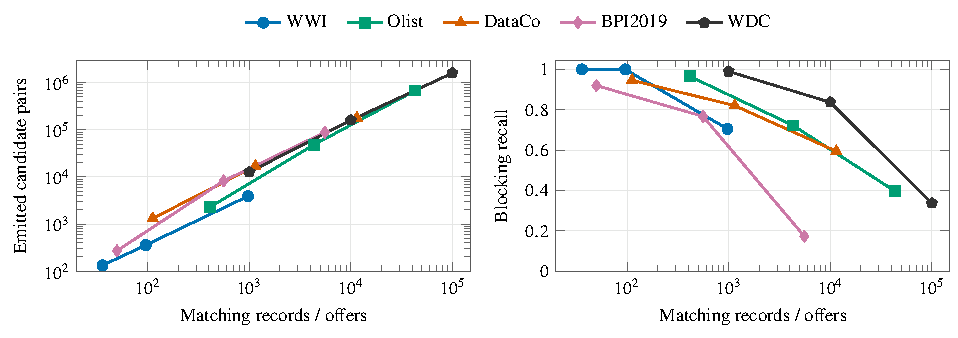
\includegraphics[width=\textwidth]{retrieval_scale.pdf}
\caption{The existing three workload points plotted against matching records/offers, not total native graph nodes. Left: emitted candidate pairs. Right: full-positive-universe blocking recall. Bounded output limits delivered pairs while replication increases the true-pair universe. These curves describe measured output and recall, not a computational complexity theorem or growth in independent entity diversity.}
\label{fig:scale}
\end{figure*}

At the largest target, blocking recall is 0.705 for WWI, 0.397 for Olist, 0.594 for DataCo, 0.172 for BPI, and 0.336 for WDC. Figure~\ref{fig:scale} shows how modestly growing capped output can coexist with substantial positive losses. Cross-replica positives increase the complete denominator; bounded postings and per-left output omit many of them. Three-point candidate slopes do not prove subquadratic internal retrieval or ranking. Completion therefore supports measured feasibility, not recall-preserving scalability.

Prepared graph execution is faster than the indexed SQLite control for the largest warmed eight-query batches: median p50 graph/SQL times are 193/768\,ms on WWI, 238/1,297\,ms on Olist, 415/1,668\,ms on DataCo, and 349/1,379\,ms on BPI. Both use the same per-copy oracle identities. Adjacency construction and SQL loading/indexing are measured separately, and five warm executions give coarse percentiles. The observation compares these implementations, not commercial optimizers, cold workloads, concurrency, or distributed engines.

Timing decomposition also limits attribution. At the largest point, Olist feature construction takes 66.777\,s and all scorers 10.919\,s; WDC blocking takes 260.016\,s and features 96.738\,s. Isolated scorer trials exclude feature construction, and supplemental WDC scorer volumes count tiled pair rows rather than offers. Neither those trials nor separately measured greedy canonicalization justify an end-to-end contextual-overhead ratio.

\section{Enterprise Applications and Implications}
\label{sec:applications}
\subsection{Procurement and Decision Auditing}
WWI connects procurement observations to inventory and supplier-finance evidence through source-supported paths and declared unit classes. The source and decision references remain available when a mistaken identity affects an answer. In seed 29, black \emph{``The Gu'' red shirt XML tag t-shirt} variants in sizes S and XXS are falsely merged with score 0.992861 against threshold 0.918069, despite four independent anchors and support 2.000. Both origins are recorded as \texttt{Warehouse.StockItems}. This case demonstrates replayable decision evidence; it is not causal feature attribution or measured human interpretability. A supportive neighborhood can coexist with a contradictory product attribute.

\subsection{Customer and Process Integration}
Olist's paired query results support account/order integration using local histories when names are unavailable. BPI supports vendor-history integration across partitioned purchase cases, but its coarse baseline and rewiring sensitivity constrain interpretation. DataCo shows that available histories can reduce both matching and downstream answer accuracy. These outcomes motivate task-specific evidence validation and continued comparison with attribute-only identities. Source amounts do not measure paid spend, and no operational intervention or human study was evaluated.

\subsection{Engineering Implications}
The linked controls separate three obligations: mapping fidelity against independent native relationships, identity quality after retrieval and constraints, and query accuracy against an oracle. SQL/graph equality verifies execution under a shared map; it cannot certify that map. The evaluated graph organizes typed paths, origins, and decisions, while equivalent relational evidence gives equivalent predictions. Postconstraint precision in Table~\ref{tab:pipeline} also exposes remaining acceptance risk, including 54 false BPI links among 372 accepted links across the three trials.

\section{Threats to Validity}
\label{sec:validity}
\subsection{Task Construction and Statistical Interpretation}
The datasets instantiate different identity tasks: simulated WWI aliases, natural Olist repeat accounts, controlled DataCo/BPI source views, and WDC offer pairs. Original source identity supplies evaluator truth; it is not independently adjudicated dirty-record truth for every task. BPI uses history-derived baseline descriptors, generic support can count missingness tags, and ablations have adapter-specific semantics. Histories are capped and canonicalization is two-source, one-to-one. Complete lineage can accompany incorrect edges; SQL and graph controls can share a mistaken mapping abstraction.

Group-before-alias splits, evaluator-only truth, training-only TF-IDF, and disjoint validation roles reduce direct leakage. They do not remove Olist's test-informed adapter amendment, small validation roles, unknown deployment prevalence, or observed WDC offer overlap. Only three seeds reuse each source population; WWI has 49 held-out entities and three suppliers. Endpoint-multiplicity bootstrap summaries and the new paired query means remain descriptive, without pooled or familywise significance claims. WDC test pools repeat across sizes. The frozen cosine is a narrow reference; fine-tuned pair matchers remain an unexecuted comparator.

Frozen-candidate stresses omit corruption effects on retrieval. Replicated scaling adds no independent entity diversity, and bounded retrieval omits positives. Five warm executions give coarse latency percentiles. Local CPU measurements and oracle-map query timings do not establish production, concurrent, distributed, or predicted-map performance. Source-unit amounts and answer-set errors do not measure financial loss or human usefulness.

\subsection{Reproducibility, Amendments, and Availability}
The original expanded study records 36 passing control tests and 3,136 verification checks, including independent metrics, all 12 graph-seed and 81 WDC frozen-score replays, and fresh query execution. This revision reruns all 36 tests and adds 748 checks for the paired query comparison, canonical links, BPI fallback diagnosis, input preservation, and all 27 WDC split cells. These checks do not constitute independent fresh-environment retraining of the expansion; the earlier primary study has a separate retraining replication.

Recorded amendments include completing interrupted WWI timing with fits preserved; deduplicating master/tag incidence for SQL Q1 and rerunning WWI E5; adding Olist seller-state paths after a test-context diagnostic before fitting; and correcting Olist transaction lineage to the order-item table, rerunning query controls and nine E5 trials without refitting. Earlier measurements and hashes remain retained, and the study is exploratory.

\textbf{Code and material availability.} The source code and supporting research materials are available on GitHub: \repositorylink. Materials include configurations, frozen policies, predictions, query definitions, results, provenance, verification reports, and editable manuscript sources. The revision supplement and executable analysis provide the paired query cells and split audit. Dataset and model acquisition follows the documented licenses; privacy-filtered derivatives and download procedures cover inputs excluded from redistribution.

\section{Conclusion}
The source-preserving architecture connects typed ingestion, traceable identity decisions, and independently controlled query execution. Exact in-scope source controls and SQL/graph evidence parity separate representation fidelity from identity accuracy. Contextual benefit is task-dependent: paired identity-query F1 improves on WWI, Olist, and BPI and declines on DataCo, while WWI transaction attribution slightly worsens. BPI's gain depends on a coarse baseline, and its absence stress exposes threshold-induced failure despite exact score fallback. Bounded retrieval also loses substantial positives as replicated workloads grow. The implemented architecture and linked controls make these limits explicit. Stronger learned references, development-selected fallback policies, informative support, recall-preserving retrieval, and independent expanded retraining remain future work.

\section*{AI Disclosure}
OpenAI GPT-6 Astra was used to enhance vocabulary, grammar, language clarity, word choice, and visuals during the preparation of this research paper. OpenAI Codex and ChatGPT also assisted with implementation, experiment orchestration, manuscript drafting and organization, bibliography management, and LaTeX formatting. The authors directed the research and remain responsible for the methods, analysis, interpretation, substantive content, and results.

\section*{Acknowledgment}
This research was partially supported by the National Science Foundation under EPSCoR Award No. OIA-1946391 and the PiLog Group. Any opinions, findings, and conclusions or recommendations expressed in this material are those of the author(s) and do not necessarily reflect the views of the National Science Foundation or the PiLog Group.

\bibliographystyle{IEEEtran}
\bibliography{references}
\end{document}
